\documentclass[journal]{IEEEtran}
\usepackage[a5paper, margin=10mm, onecolumn]{geometry}
\usepackage{lmodern}
\usepackage{tfrupee}
\setlength{\headheight}{1cm}
\setlength{\headsep}{0mm}

\usepackage{gvv-book}
\usepackage{gvv}
\usepackage{cite}
\usepackage{amsmath,amssymb,amsfonts,amsthm}
\usepackage{algorithmic}
\usepackage{graphicx}
\usepackage{textcomp}
\usepackage{xcolor}
\usepackage{txfonts}
\usepackage{listings}
\usepackage{enumitem}
\usepackage{mathtools}
\usepackage{gensymb}
\usepackage{comment}
\usepackage[breaklinks=true]{hyperref}
\usepackage{tkz-euclide}
\usepackage{listings}
\def\inputGnumericTable{}
\usepackage[latin1]{inputenc}
\colorlet{punct}{red!60!black}
\definecolor{background}{HTML}{EEEEEE}
\definecolor{delim}{RGB}{20,105,176}
\colorlet{sqbracket}{delim}
\colorlet{comment}{green!50!black}
\usepackage{array}
\usepackage{longtable}
\usepackage{calc}
\usepackage{multirow}
\usepackage{hhline}
\usepackage{ifthen}
\usepackage{lscape}
\usepackage{xparse}

\bibliographystyle{IEEEtran}

\title{2.4.40}
\author{EE25BTECH11043 - Nishid Khandagre}
\begin{document}
\maketitle

\renewcommand{\thefigure}{\theenumi}
\renewcommand{\thetable}{\theenumi}

\numberwithin{equation}{enumi}
\numberwithin{figure}{enumi}

\textbf{Question}:\
Find the angle between the lines $-\sqrt{3}x + y - 5 = 0$ and $- x + \sqrt{3}y + 6 = 0$.

\textbf{Solution: }
Given lines:
\begin{align}
L_1: -\sqrt{3}x + y - 5 &= 0 \\
L_2: - x + \sqrt{3}y + 6 &= 0
\end{align}

The matrix form of a line can be written as \\ 
\begin{align}
\vec{n}^\top \vec{x} = C
\end{align}
Where $\vec{n}$ is the normal vector and $\vec{x} = \myvec{x \\ y}$ is the position vector.


\begin{align}
L_1: \vec{n_1}^\top\vec{x}&=c_1\\
L_2: \vec{n_2}^\top\vec{x}&=c_2
\end{align}

Where $\vec{n_1}$ and $\vec{n_2}$ are the normal vectors to the lines $L_1$ and $L_2$ respectively.
\begin{align}
\vec{n_1} &= \myvec{-\sqrt{3} \\ 1} \\
\vec{n_2} &= \myvec{-1 \\ \sqrt{3}}
\end{align}

The angle $\theta$ between the lines is the angle between their normal vectors.
\begin{align}
\cos \theta = \frac{\vec{n_1}^\top \vec{n_2}}{\norm{\vec{n_1}} \norm{\vec{n_2}}} \label{eq:equation}
\end{align}



\begin{align}
\vec{n_1}^\top \vec{n_2} &= \myvec{ -\sqrt{3} & 1 } \myvec{-1 \\ \sqrt{3}} \\
&= (-\sqrt{3})(-1) + (1)(\sqrt{3}) \\
&= 2\sqrt{3}
\end{align}


\begin{align}
\norm{\vec{n_1}} &= \sqrt{\vec{n_1}^\top\vec{n_1}}\\
&= \sqrt{(-\sqrt{3})^2 + (1)^2} \\
&= \sqrt{4} \\
&= 2
\end{align}

\begin{align}
\norm{\vec{n_2}} &= \sqrt{\vec{n_2}^\top\vec{n_2}}\\
&= \sqrt{(-1)^2 + (\sqrt{3})^2} \\
&= \sqrt{4} \\
&= 2
\end{align}

Now, substitute these values into the formula \eqref{eq:equation}
\begin{align}
\cos \theta &= \frac{2\sqrt{3}}{(2)(2)} \\
&= \frac{\sqrt{3}}{2}
\end{align}

\begin{align}
\theta &= \frac{\pi}{6} \text{ radians}
\end{align}


\begin{figure}[H]
\centering
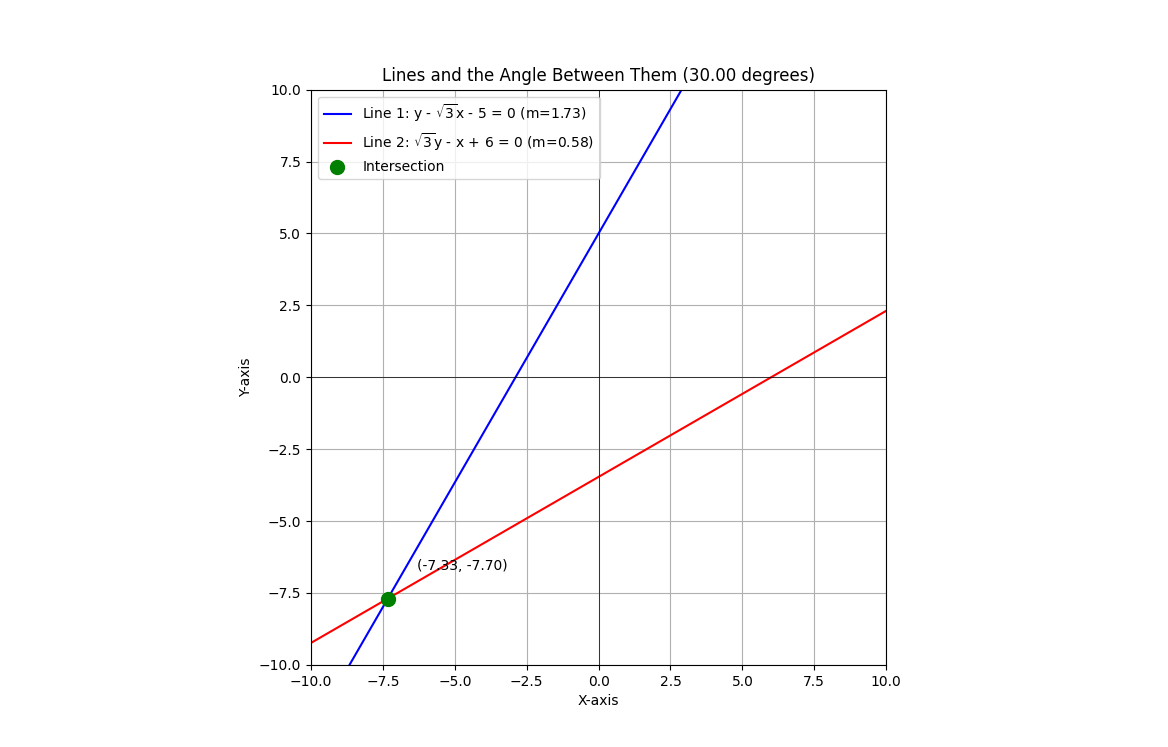
\includegraphics[width=0.9\columnwidth]{figs/fig1.png}
\caption{}
\label{fig:1}
\end{figure}

\end{document}
